\chapter{Data-driven results}\label{ch:data-driven-results}
In this chapter we present the results of the data-driven models, that is, the convolutional neural network (CNN) and the Fourier neural operator (FNO), for solving the shallow water equations.
We analyse three main cases:
\begin{enumerate}
    \item 1D SWE with Gaussian initial conditions. 
    \item 1D LSWE in spherical coordinates.
    \item 2D SWE with Gaussian initial conditions.
\end{enumerate}
In each case, we evaluate the performance of the CNN and the FNO in terms of mean squared error (MSE), mean absolute error (MAE), training time and prediction time.
In addition, we analyze the models' predictions for various initial conditions and their ability to generalize to unseen data.
We also explore their capability to transfer solutions aross grid resolutions, such as transitioning from coarse to fine grids.
Lastly, we evaluate the models' long-term predictive performance, assessing how well they maintain accuracy over extended time steps.
In the end of the chapter, we provide a concise summary of the results.
The CNNs are implemented in python version 3.12.6, using PyTorch version 2.4.1.
The FNOs are implemented using the Github repository \textit{neuraloperator}, which is a library for learning neural operators in PyTorch~\cite{neuraloperator}.

In \autoref{ch:numerical_results}, we presented the results of discontinuous test cases, operating under the premise that a solver capable of handling discontinuous solutions should also perform well with smooth solutions.
In this chapter, we focus on evaluating the performance of data-driven models under smooth initial conditions, as they provide a more suitable starting point.

\section{The 1D Shallow Water Equations with Gaussian initial conditions}\label{sec:data-driven-results-1D}
In this section, we consider the 1D SWE with Gaussian initial conditions, where the data is generated as described in \autoref{sec:data_generation_fvm}.
The initial condition for the water height $h$ is given in~\eqref{eq:1D_swe_ic_gaussian} and illustrated in \autoref{fig:NN_initial_1D}.
\begin{figure}[H]
    \centering
    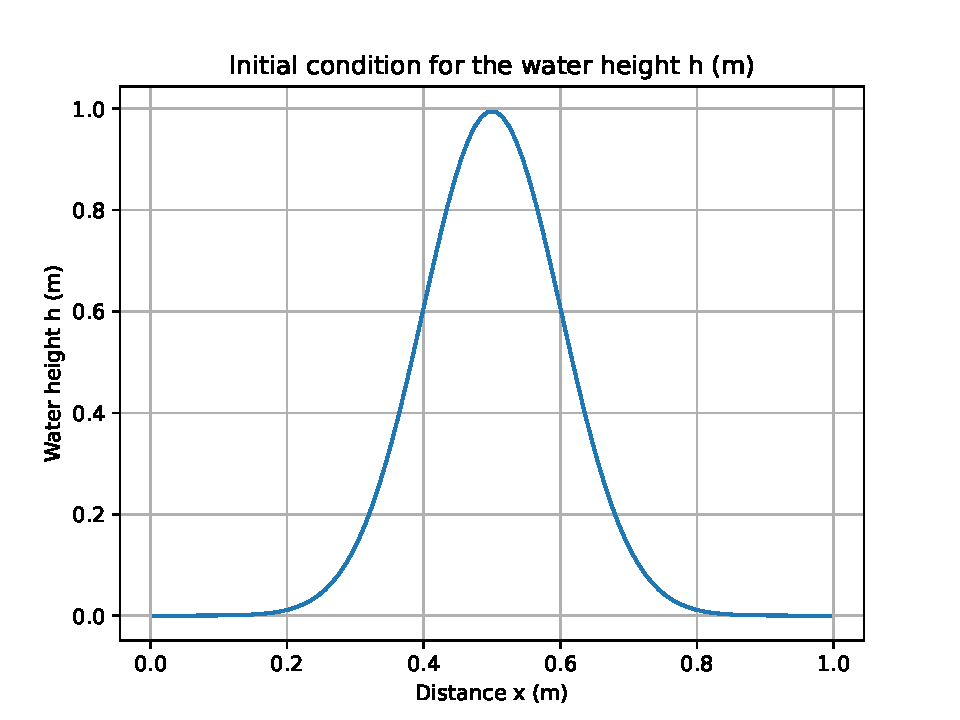
\includegraphics[width=0.4\textwidth]{C:/Users/Matteo/Shallow-Water-Equations/plots/NN_initial_1D.pdf}
    \caption{The initial conditions for the water level $h$ in the 1D SWE.}\label{fig:NN_initial_1D}
\end{figure}
The domain is $ x \in [0, 1]$ m and the data covers the time interval $t \in [0, 1]$ s.
In \autoref{fig:NN_initial_1D}, we see that the initial condition is a Gaussian function with center in the middle of the domain.
To get an overview of how the solution evolves over time, we have plotted the numerical solution in the $x,t-$plane, shown in \autoref{fig:NN_initial}, in both a contour plot and a 3D plot.
\begin{figure}[H]
    %\centering
    \hspace{1.7cm} % Adjust the spacing as needed
    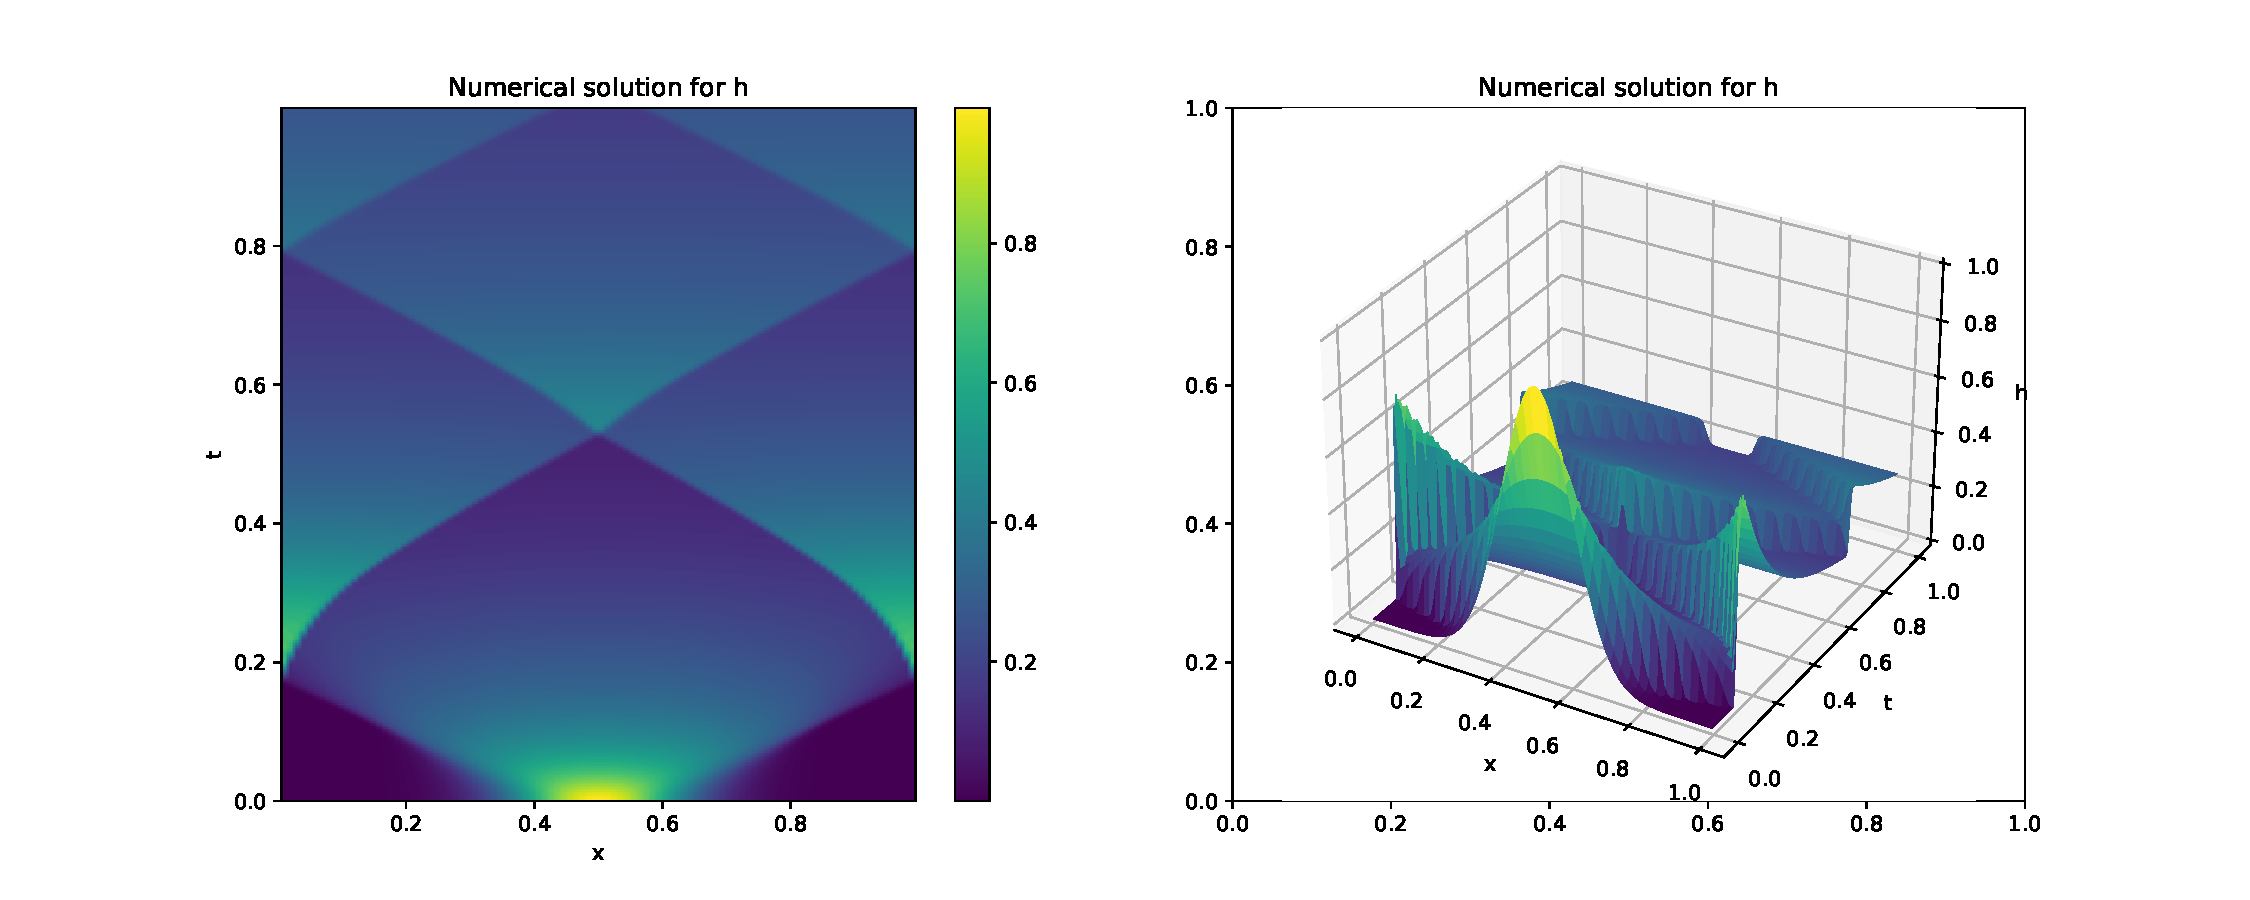
\includegraphics[width=0.95\textwidth]{C:/Users/Matteo/Shallow-Water-Equations/plots/NN_initial.pdf}
    \caption{Numerical solution of the 1D SWE from $t = 0$ s to $t = 1$ s.}\label{fig:NN_initial}
\end{figure}
In \autoref{fig:NN_initial}, we see how the water height in the domain evolves over time.
The 3D plot provides an overview of the solution, whereas the contour plot offers a more detailed view of the water levels.
From the contour plot, we observe that even though the initial condition is smooth, the solution develops sharp edges, close to discontinuities, over time, represented by the lines in the plot.
This behavior is typical for the nonlinear shallow water equations, where the solution tend to develop discontinuities due to the formation of shock waves.
Some details of the data cen be seen in the following table.
\begin{table}[H]
    \centering
    \begin{tabular}{c|cccccc}
        \textbf{Case} & \textbf{n\_train} & \textbf{n\_val} & \textbf{n\_test} & \textbf{N} & $\mathbf{\Delta x}$ & $\mathbf{\Delta t}$ \\
        \hline
        1D SWE & 369 & 123 & 123 & 200 & 0.005 m & $[0.0008 \text{ s}, 0.00225 \text{ s}]$ \\
    \end{tabular}
    \caption{Details of the used data for the case with the 1D SWE with a Gaussian initial condition.}\label{tab:cnn_data}
\end{table}
In \autoref{tab:cnn_data}, there are listed some details of the CNN model.
The time step size $\Delta t$ is not constant, but varies between $0.0008$ s and $0.00225$ s.
This is due to the CFL condition, which requires the time step size to be small enough to ensure stability.


\subsection*{CNN Model}
In the convolutional neural network, we train the model using the generated data.
The input and output data are the same, shifted by one time step, allowing the model to predict the solution at the next time step.
This approach enables the model to learn the flowmap, as described in~\autoref{sec:CNN}.
The model takes input with 10 channels, corresponding to the sequence length, and processes it through a series of three 1D convolutional layers with ReLU activation functions.
The final convolutional layer reduces the output to a single channel, which is then mapped to the prediction using a fully connected layer.
Training is performed using the Adam optimizer with a learning rate of $0.001$ and a batch size of $32$.
The loss function minimizes the mean squared error (MSE).
The data set is split into $60\%$ training, $20\%$ validation, and $20\%$ testing data, with the exact number of training points provided in \autoref{tab:cnn_data}.
The model is trained for 500 epochs, where the model's parameters are continuous saved if the validation loss improves upon the previous best.
This is done to prevent overfitting.
The training and validation losses for the CNN model are shown in \autoref{fig:1D_CNN_loss}.
\begin{figure}[H]
    \centering
    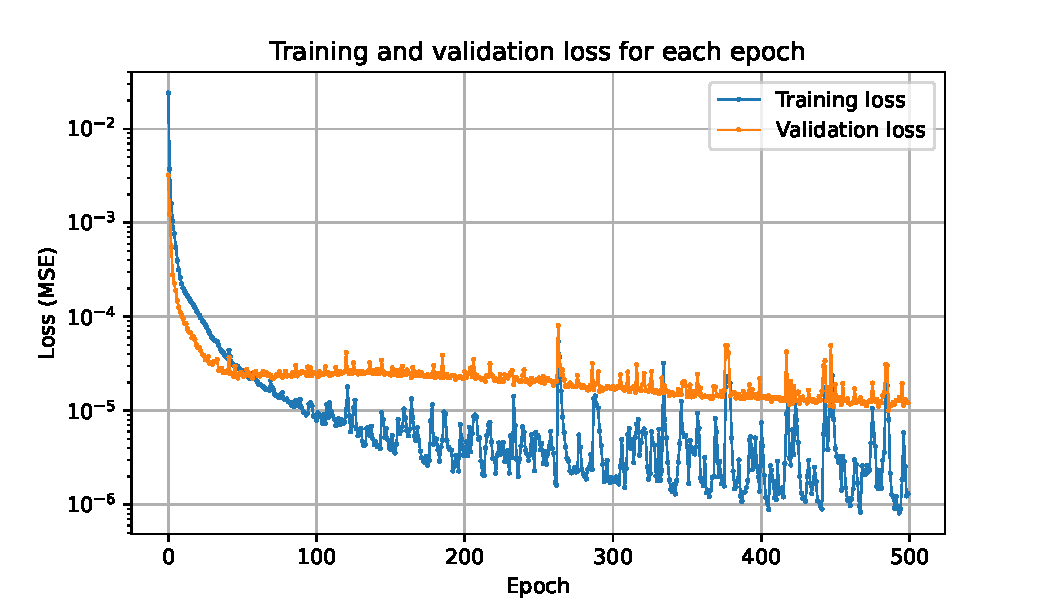
\includegraphics[width=0.7\textwidth]{C:/Users/Matteo/Shallow-Water-Equations/plots/1D_CNN_loss.pdf}
    \caption{Training and validation loss (MSE) for the CNN model.}\label{fig:1D_CNN_loss}
\end{figure}
In \autoref{fig:1D_CNN_loss}, we see that the training and validation loss decrease over the epochs, demonstrating that the model is learning the dynamics of the solution.
However, while the training loss continues to decrease, the validation loss has largely stabilized.
This indicates that further training is unlikely to improve the model's performance and may lead to overfitting.
Additionally, we assess the accuracy of the model's predictions by examining the error, as shown in \autoref{fig:1D_CNN_error}.
\begin{figure}[H]
    \centering
    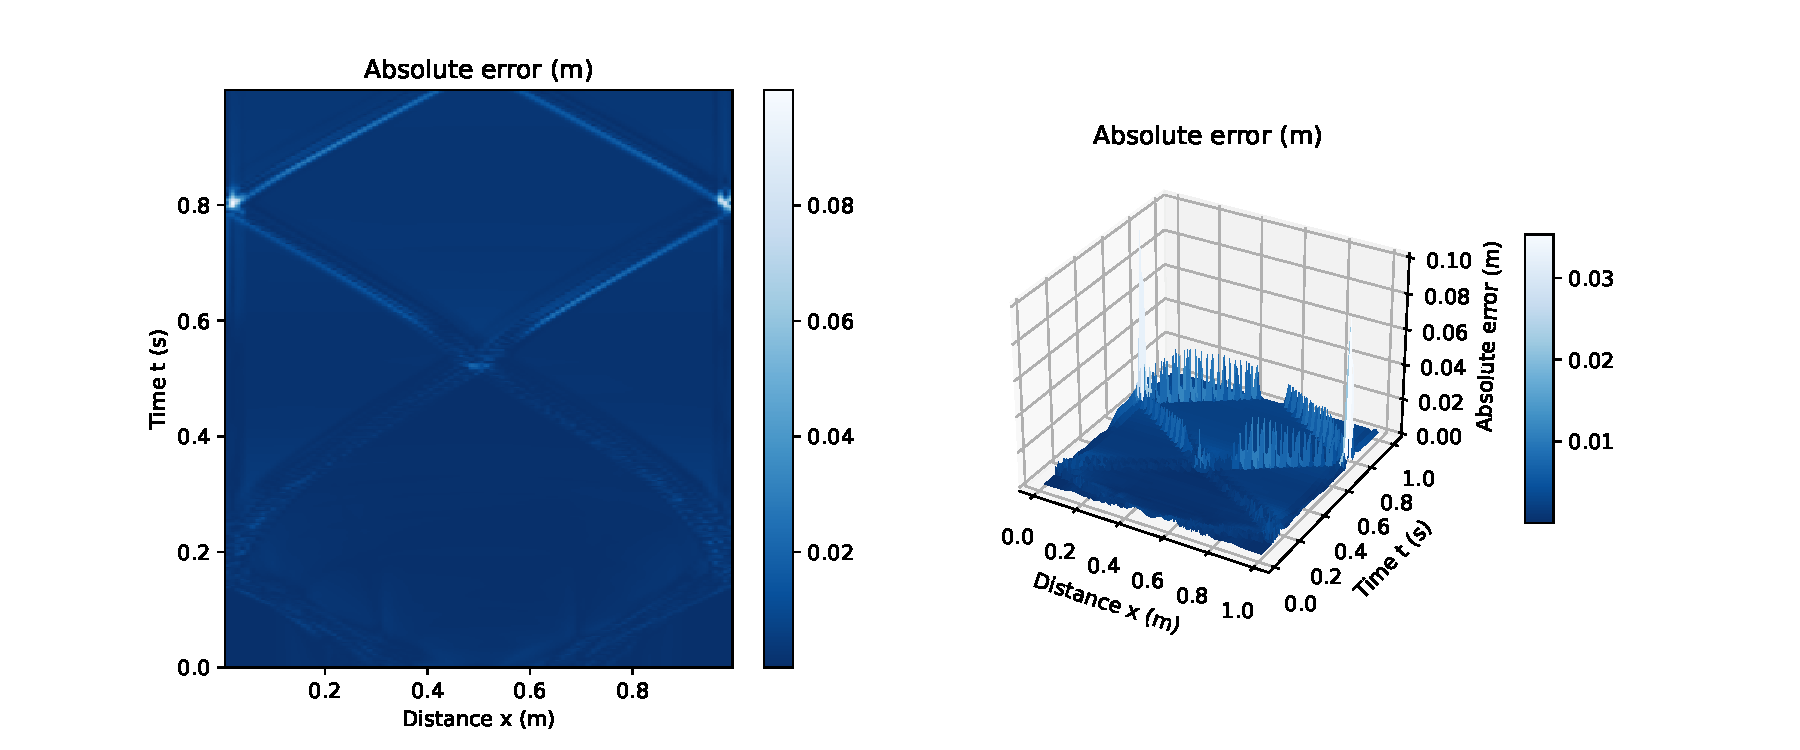
\includegraphics[width=\textwidth]{C:/Users/Matteo/Shallow-Water-Equations/plots/1D_CNN_error.pdf}
    \caption{Error plot for the predictions for the CNN model.}\label{fig:1D_CNN_error}
\end{figure}
From \autoref{fig:1D_CNN_error}, we see that the largest errors are observed in regions where the solution exhibits discontinuities, which is expected as the model struggles to make accurate predictions in these areas.
To gain deeper insight into the model's performance, we examine its predictions at specific time steps, as shown in \autoref{fig:1D_CNN_pred_timesteps}.
\begin{figure}[H]
    \centering
    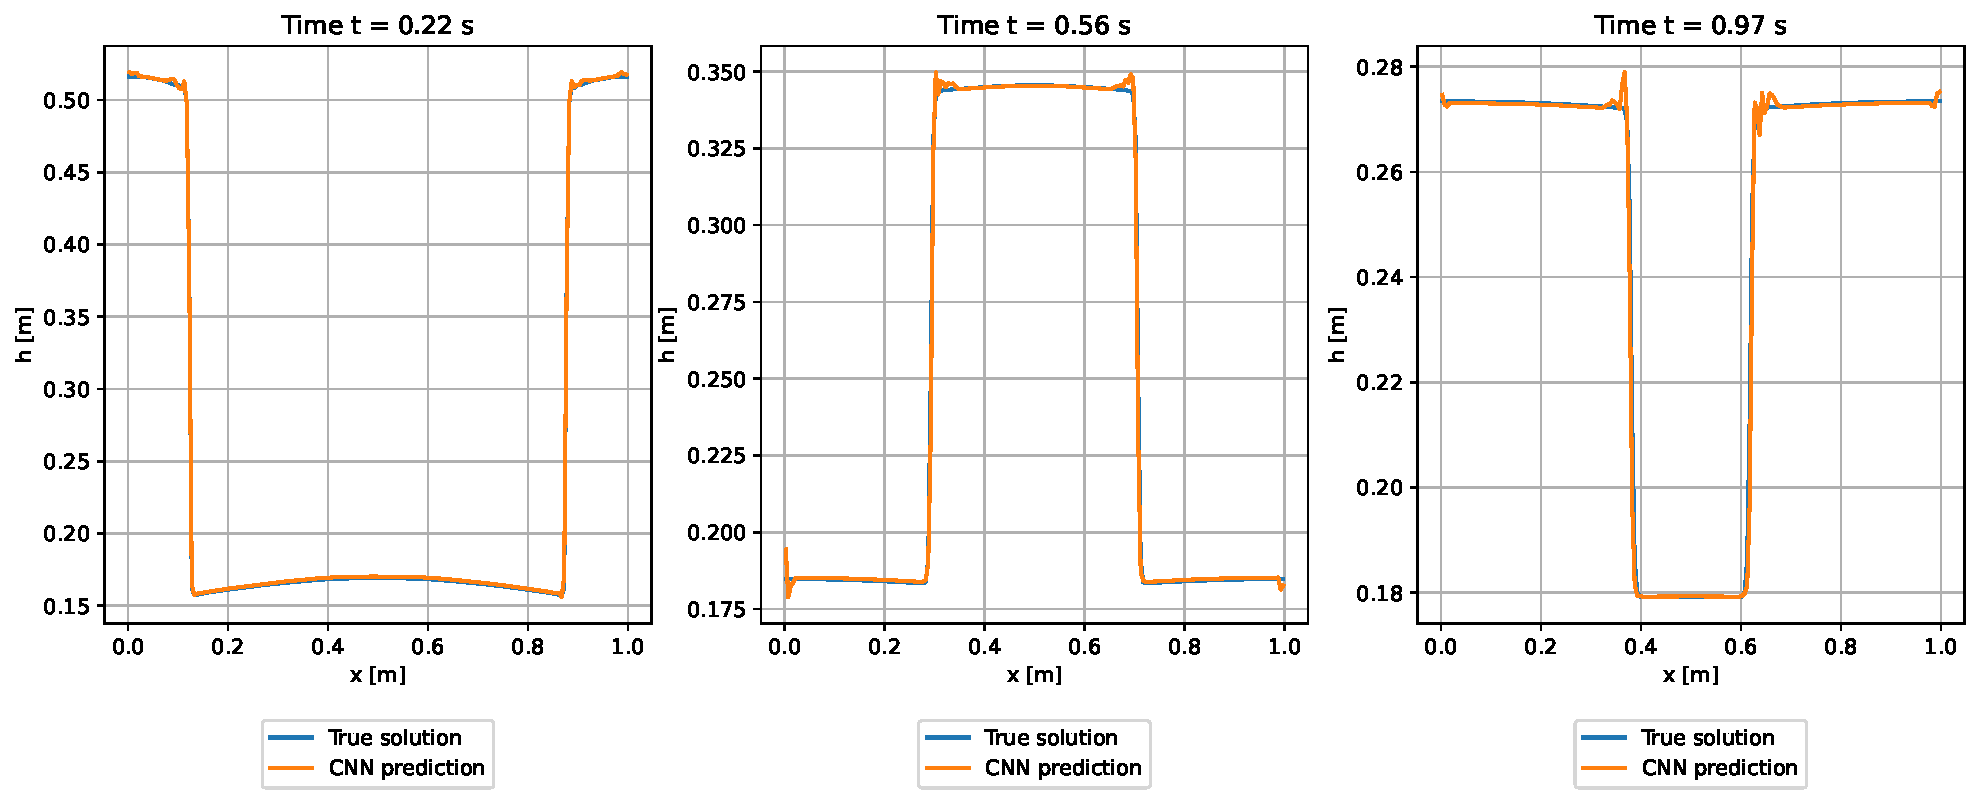
\includegraphics[width=\textwidth]{C:/Users/Matteo/Shallow-Water-Equations/plots/1D_CNN_pred_timesteps.pdf}
    \caption{Predictions for the CNN model for some given time steps.}\label{fig:1D_CNN_pred_timesteps}
\end{figure}
From \autoref{fig:1D_CNN_pred_timesteps}, we observe that the CNN model overall captures the dynamics of the solution, but struggles to predict the sharp edges.
This is especially illustrated in the prediction at $t = 0.97$ s, where we observe oscillations in the solution that are not present in the true solution.

\subsection*{FNO Model}
We define a FNO model, which consists of an input channel, 64 hidden channels and an output channel. We use a Fourier basis with 16 modes and a batch size of 32.
The model is trained using the Adam optimizer with a learning rate of $0.001$ and the critera is to minimize the mean squared error (MSE).
We use the same train/validation/test split as for the CNN model.
The model is trained for $500$ epochs, but the current best model is saved if the validation loss is lower than the previous best validation loss.
The training and validation loss for the FNO model is shown in \autoref{fig:1D_FNO_loss}.
\begin{figure}[H]
    \centering
    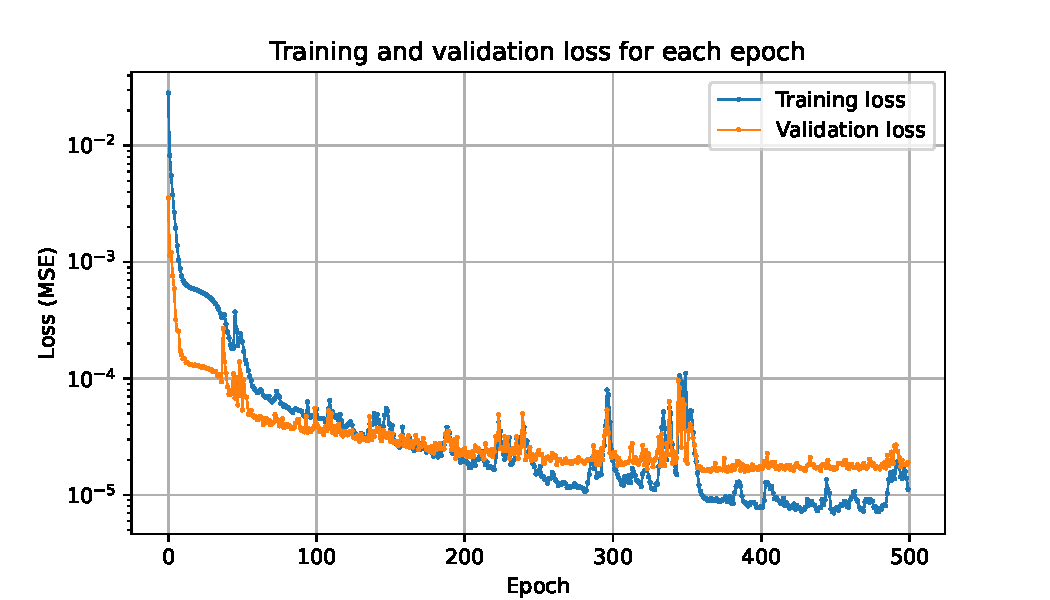
\includegraphics[width=0.7\textwidth]{C:/Users/Matteo/Shallow-Water-Equations/plots/1D_FNO_loss.pdf}
    \caption{Training and validation loss for the FNO model.}\label{fig:1D_FNO_loss}
\end{figure}
From \autoref{fig:1D_FNO_loss}, we see that the training and validation loss decrease over the epochs, indicating that the model is learning the dynamics of the solution.
The losses drop quickly and are then more or less stable, suggesting that further training is unlikely to improve the model's performance.
To see how the errors are distributed in the solution, we plot the error in \autoref{fig:1D_FNO_error}.
\begin{figure}[H]
    \centering
    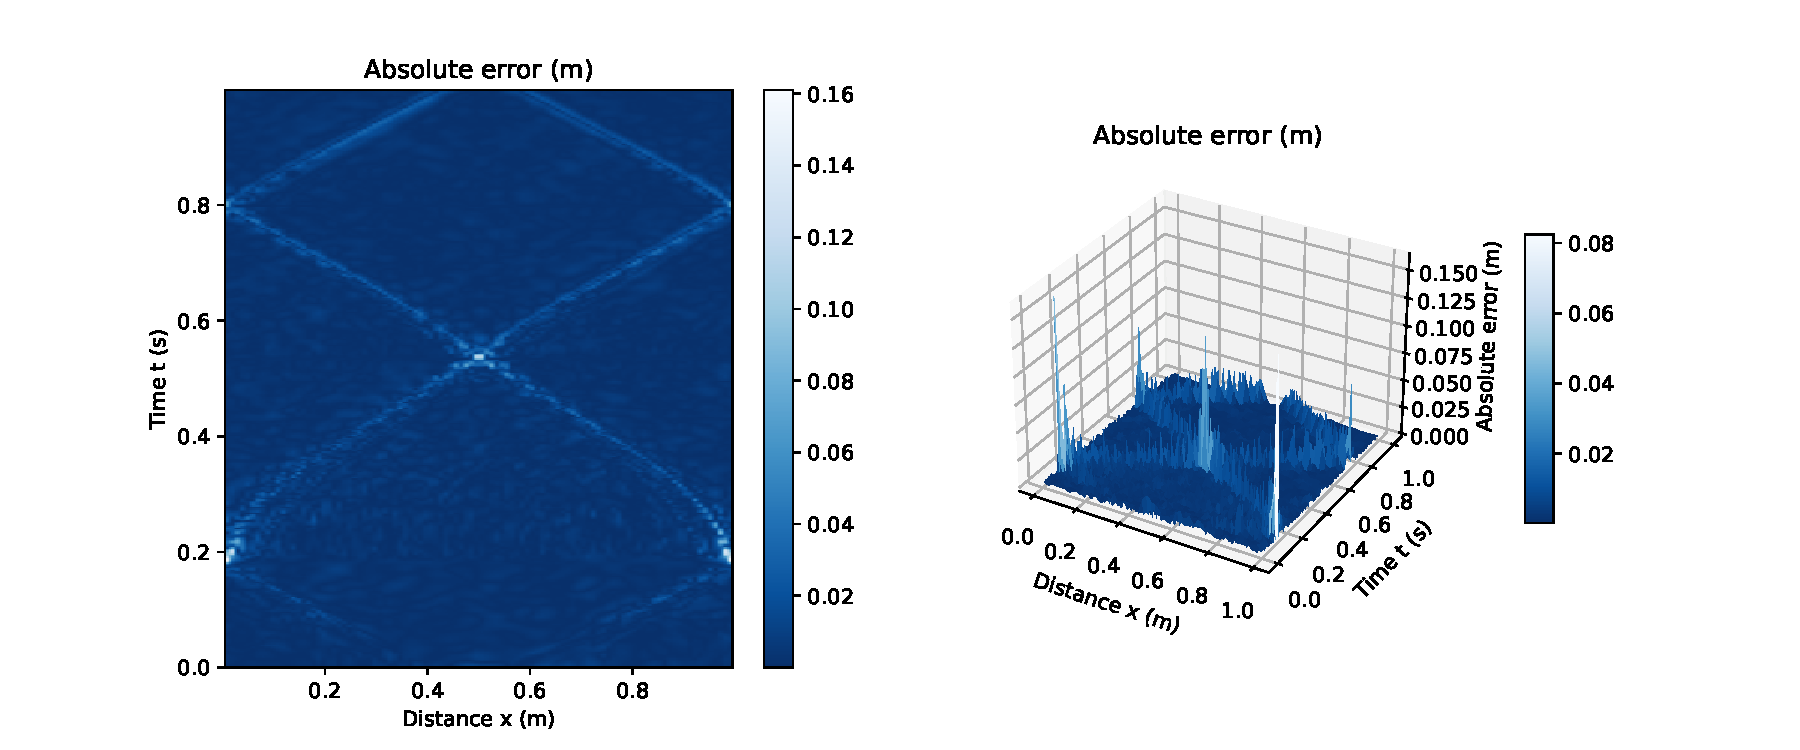
\includegraphics[width=\textwidth]{C:/Users/Matteo/Shallow-Water-Equations/plots/1D_FNO_error.pdf}
    \caption{Error plot for the predictions for the FNO model.}\label{fig:1D_FNO_error}
\end{figure}
In \autoref{fig:1D_FNO_error}, we see more or less the same error distribution as for the CNN model, with the largest errors at the discontinuities.
We also consider the predictions for some given time steps, shown in \autoref{fig:1D_FNO_pred_timesteps}.
\begin{figure}[H]
    \centering
    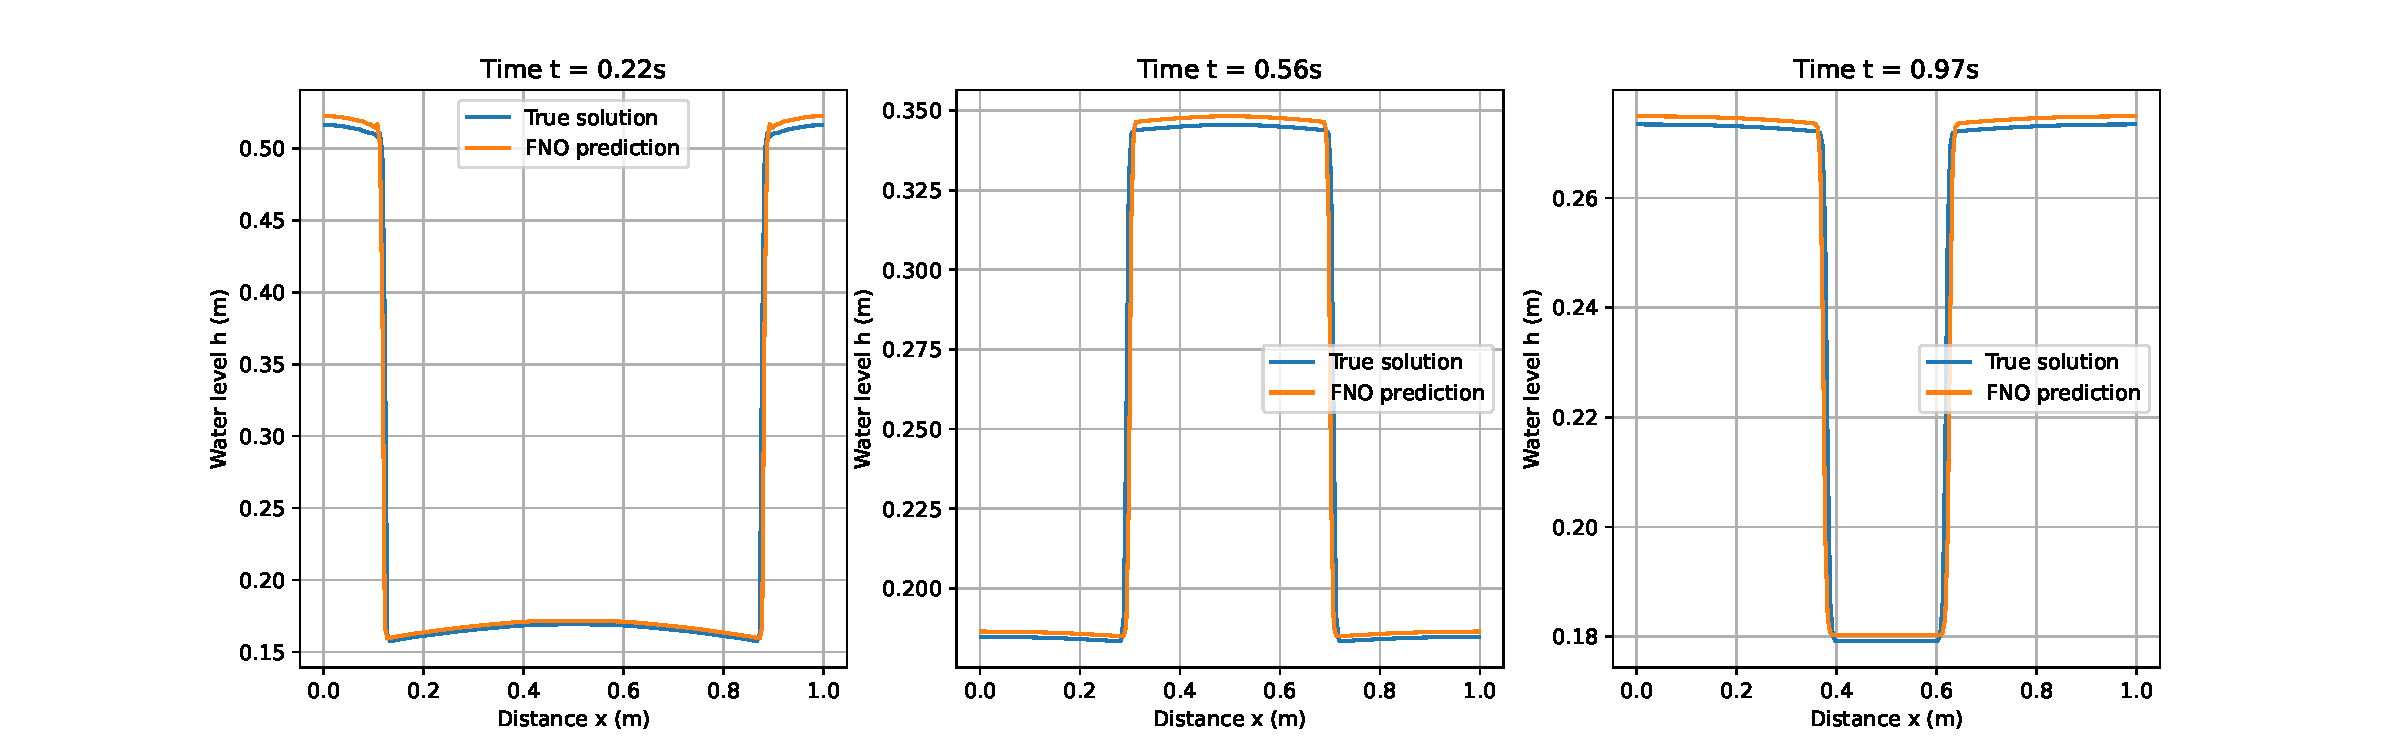
\includegraphics[width=\textwidth]{C:/Users/Matteo/Shallow-Water-Equations/plots/1D_FNO_pred_timesteps.pdf}
    \caption{Predictions for the FNO model for some given time steps.}\label{fig:1D_FNO_pred_timesteps}
\end{figure}
From \autoref{fig:1D_FNO_pred_timesteps}, we see that the FNO model produces smooth predictions, avoiding the oscillations seen in the CNN model.
However the FNO model shows general inaccuracies in the solution.

\subsection*{New initial condition}
To evaluate the models' ability to generalize to unseen data, we introduce a new initial condition for the water height $h$.
This new condition retains the Gaussian form described in~\eqref{eq:1D_swe_ic_gaussian}, but with a different mean parameter $\mu$.
Specifically, $\mu$ is set to $\mu = 0.3$ m, shifting the initial condition to the left.
The new initial condition is illustrated in \autoref{fig:1D_new_ic}.
\begin{figure}[H]
    \centering
    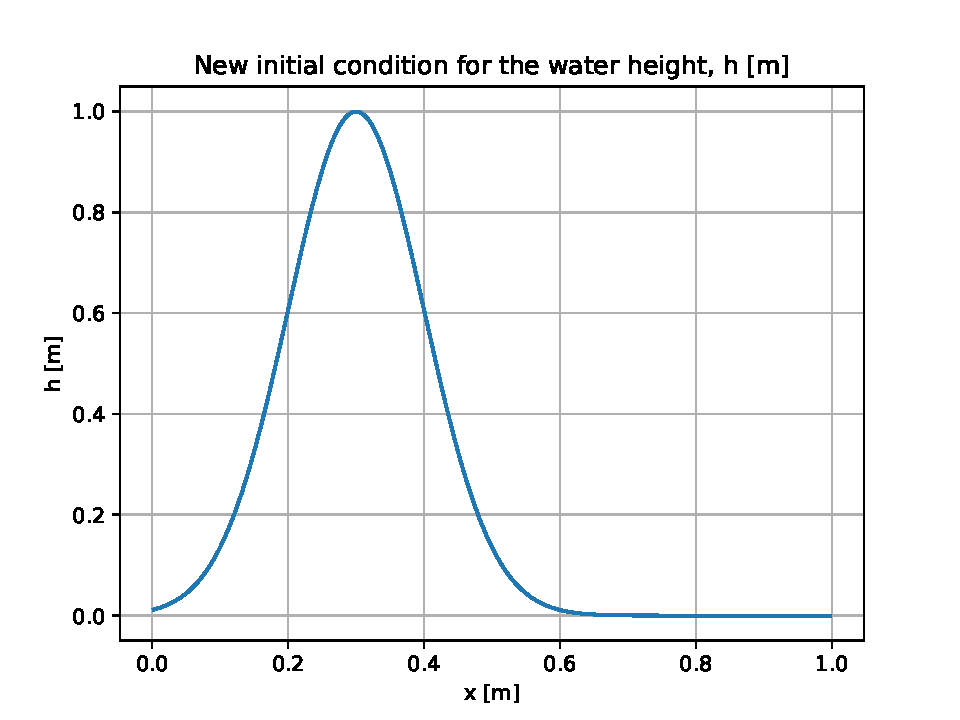
\includegraphics[width=0.5\textwidth]{C:/Users/Matteo/Shallow-Water-Equations/plots/1D_new_ic.pdf}
    \caption{New initial condition for the 1D SWE.}\label{fig:1D_new_ic}
\end{figure}
The models are then tasked with making predictions for the new initial condition without retraining.
These predictions cover a single time step, and the results are summarized in \autoref{tab:results_1D_comparison}.

\subsection*{Comparison}
To compare the performance of the CNN and FNO models, we evaluate the MSE and MAE for the test data predictions of the 1D SWE, with Gaussian initial conditions of $\mu = 0.5$ m, as well as for the new initial condition with $\mu = 0.3$ m.
The reason we consider both MSE and MAE is that the MSE is more sensitive to outliers, while the MAE provides a more general overview of the error.
The results are summarized in \autoref{tab:results_1D_comparison}.
\begin{table}[H]
    \centering
    \small % Reduce font size
    \begin{tabular}{c|cccc|ccc}
        Model & \multicolumn{4}{c|}{Gauss initial condition} & \multicolumn{3}{c}{New initial condition} \\
        \cline{2-8}
        & Epochs & MSE & MAE & Training time [s]  & MSE & MAE & Prediction time [s] \\
        \hline
        CNN  &
        \input{C:/Users/Matteo/Shallow-Water-Equations/saved_results/1D_CNN_nepochs.txt} &
        \input{C:/Users/Matteo/Shallow-Water-Equations/saved_results/1D_CNN_MSE_test.txt} & 
        \input{C:/Users/Matteo/Shallow-Water-Equations/saved_results/1D_CNN_MAE_test.txt} &
        \input{C:/Users/Matteo/Shallow-Water-Equations/saved_results/1D_CNN_time.txt} &
        \input{C:/Users/Matteo/Shallow-Water-Equations/saved_results/1D_CNN_MSE_test_new_ic.txt} &
        \input{C:/Users/Matteo/Shallow-Water-Equations/saved_results/1D_CNN_MAE_test_new_ic.txt} &
        \input{C:/Users/Matteo/Shallow-Water-Equations/saved_results/1D_CNN_time_new_ic.txt} 
        \\
        \hline
        FNO  &
        \input{C:/Users/Matteo/Shallow-Water-Equations/saved_results/1D_FNO_nepochs.txt} &
        \input{C:/Users/Matteo/Shallow-Water-Equations/saved_results/1D_FNO_MSE_test.txt} &
        \input{C:/Users/Matteo/Shallow-Water-Equations/saved_results/1D_FNO_MAE_test.txt} &
        \input{C:/Users/Matteo/Shallow-Water-Equations/saved_results/1D_FNO_time.txt} &
        \input{C:/Users/Matteo/Shallow-Water-Equations/saved_results/1D_FNO_MSE_test_new_ic.txt} &
        \input{C:/Users/Matteo/Shallow-Water-Equations/saved_results/1D_FNO_MAE_test_new_ic.txt} &
        \input{C:/Users/Matteo/Shallow-Water-Equations/saved_results/1D_FNO_time_newic.txt}
        \\
        \hline
    \end{tabular}
    \caption{Test loss in terms of MSE and MAE, and time for training the models for the 2D SWE.}\label{tab:results_1D_comparison}
\end{table}
From \autoref{tab:results_1D_comparison}, we observe that both models achieve a low MSE and MAE for the Gaussian initial conditions, indicating strong performance.
However, the training time for the FNO model is significantly higher than that of the CNN model.
For the new initial condition, the FNO model maintains a low MSE and MAE, whereas the CNN model exhibits increased error.
Since the CNN model initally outperformed the FNO model in terms of error, the two models now have nearly identical errors for the new initial condition.

\section{The 1D linearized Shallow Water Equations in Spherical Coordinates}
In this section, we consider the 1D LSWE in spherical coordinates on a circular domain.
The length of the domain corresponds to the circumreference of the circle, $L = 2\pi$ m, and is discretized into $N = 500$ points.
The initial condition for the water height is specified as a Gaussian function wrapped around the circle as given in~\eqref{eq:1D_swe_spherical_ic}.
We use the middle value of $\sigma$, i.e., $\sigma = \frac{\pi}{16}$, to generate the initial conditions.
The initial conditions can be seen in \autoref{fig:swe_spherical_1d_initial_conditions}.
To get an overview of how the solution evolves, we have plotted the numerical solution in the $\theta,t-$plane from $t = 0$ s to $t = 1.0$ s, shown in \autoref{fig:Spherical_linear_1D_true_solution}.
\begin{figure}[H]
    \centering
    \begin{subfigure}[t]{0.4\textwidth} % Align top
        \centering
        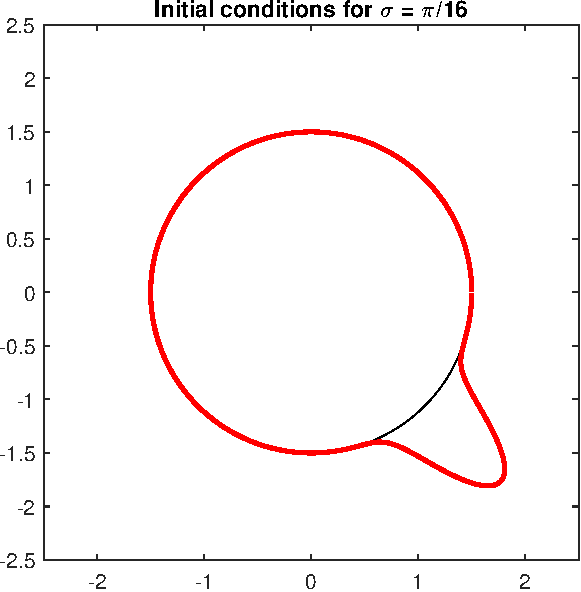
\includegraphics[width=0.8\textwidth]{C:/Users/Matteo/Shallow-Water-Equations/plots/SWE-spherical-1d-initial_conditions_sigma2.pdf}
        \caption{Initial conditions for the 1D LSWE on a sphere.}\label{fig:swe_spherical_1d_initial_conditions}
    \end{subfigure}
    \hspace{0mm} % Adjust the spacing as needed
    \begin{subfigure}[t]{0.5\textwidth} % Align top
        \centering
        %\raisebox{0mm}{
        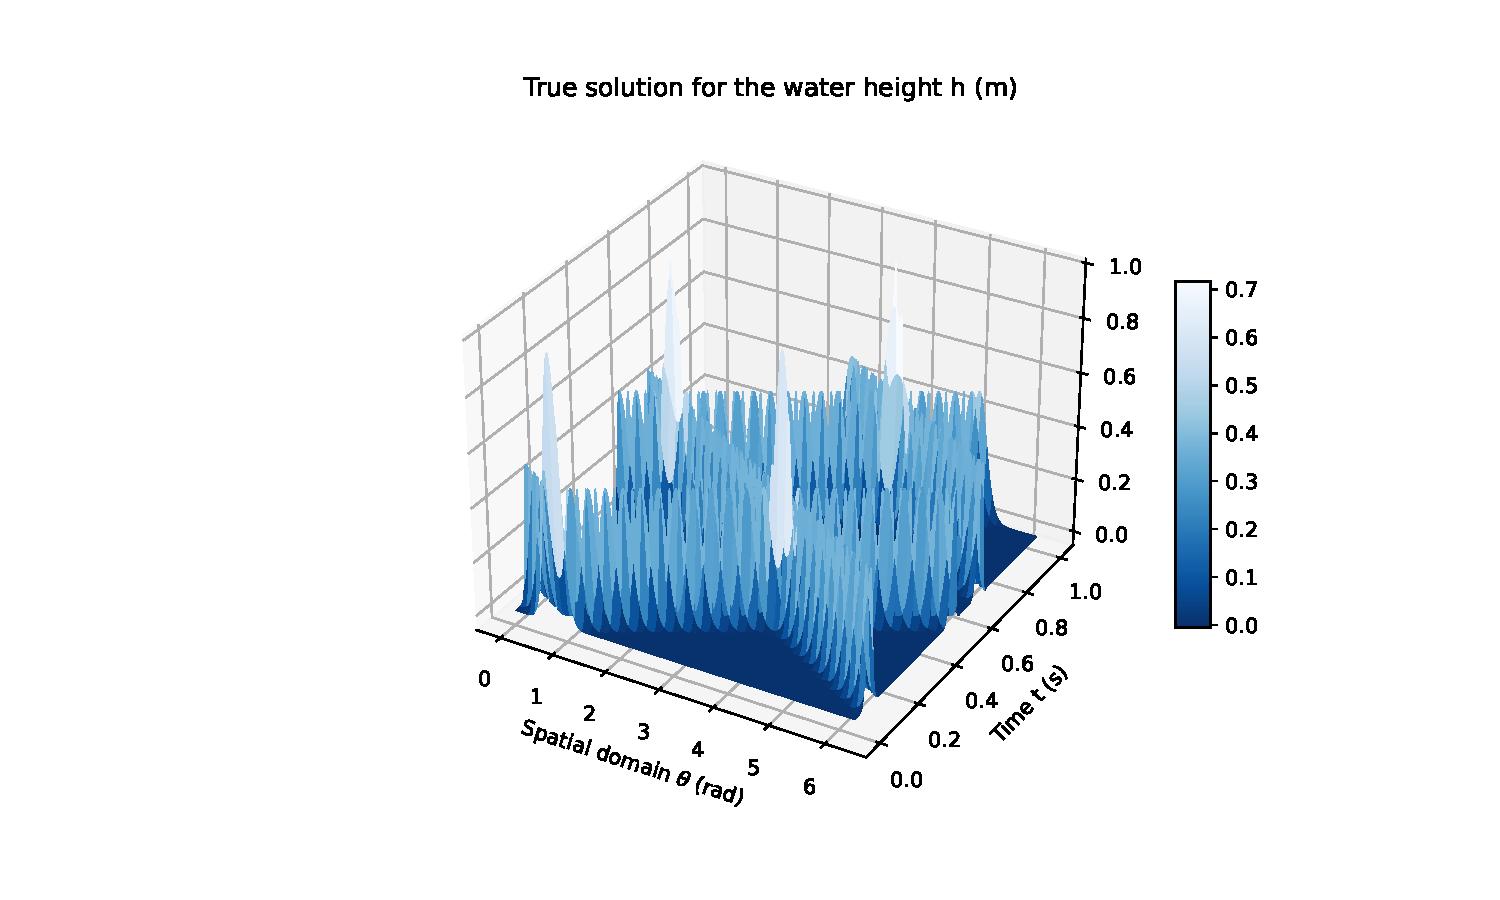
\includegraphics[width=\textwidth]{C:/Users/Matteo/Shallow-Water-Equations/plots/Spherical_linear_1D_true_solution.pdf}
        %}
        \caption{Numerical solution of the 1D spherical LSWE in the $\theta,t-$space.}\label{fig:Spherical_linear_1D_true_solution}
    \end{subfigure}
    \caption{Visualization of the 1D LSWE on a sphere:
    (a) shows the initial conditions, and (b) presents the numerical solution.}\label{fig:LSWE_1D_sphere}
\end{figure}
In \autoref{fig:Spherical_linear_1D_true_solution}, we see that the solution has some steep descents, and it is interesting to see how the data-driven models handle these sharp edges.
Some details of the data such as the number of training, validation and test points, and the grid spacing can be seen in \autoref{tab:data_1D_LSWE}.
\begin{table}[H]
    \centering
    \begin{tabular}{c|cccccc}
        \textbf{Case} & \textbf{n\_train} & \textbf{n\_val} & \textbf{n\_test} & \textbf{N} & $\mathbf{\Delta \theta}$ & $\mathbf{\Delta t}$ \\
        \hline
        1D spherical LSWE & 240 & 80 & 81 & 500 & $\frac{2 \pi}{500} = 0.0126$ rad  & 0.0025 s \\
    \end{tabular}
    \caption{Details of the used data for the case with the 1D LSWE in spherical coordinates.}\label{tab:data_1D_LSWE}
\end{table}
In \autoref{tab:data_1D_LSWE}, we see that in constrast to the 1D SWE, the time step size $\Delta t$ is constant.
From the number of training, validation and test points, we see that the data is split into $60\%$ training, $20\%$ validation and $20\%$ test data, like for the 1D SWE with Gaussian initial conditions.

\subsubsection*{CNN Model}
We define and train a CNN model to solve the spherical 1D LSWE.
The model takes input with 10 channels, corresponding to the sequence length, and processes it through a series of three 1D convolutional layers with ReLU activation functions.
The criteria is to minimize the MSE, and the model is trained using the Adam optimizer with a learning rate of $0.001$ and a batch size of $32$.
Training is conducted over $500$ epochs, continuously saving the current best model.
The training and validation loss is shown in \autoref{fig:1D_CNN_sphere_loss}.
\begin{figure}[H]
    \centering
    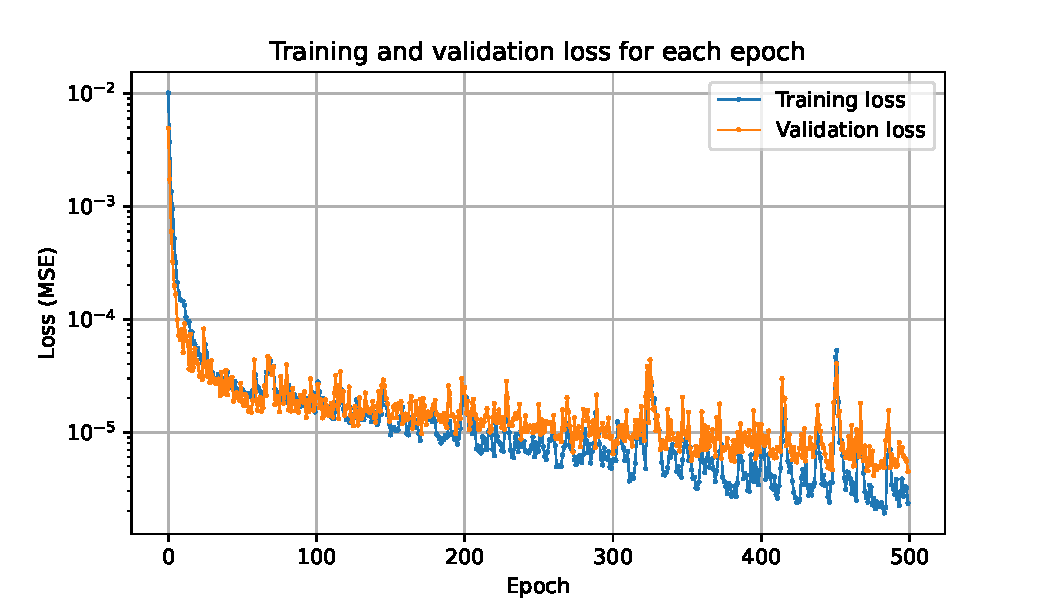
\includegraphics[width=0.7\textwidth]{C:/Users/Matteo/Shallow-Water-Equations/plots/1D_CNN_sphere_loss.pdf}
    \caption{Training and validation loss for the CNN model for the 1D spherical LSWE.}\label{fig:1D_CNN_sphere_loss}
\end{figure}
In \autoref{fig:1D_CNN_sphere_loss}, we see that the training and validation loss decrease over the epochs, indicating that the model is learning the dynamics of the solution.
We note that the cross between the training and validation loss is quite early, which we also observed for the CNN model in the case with the 1D SWE with Gaussian initial conditions.
To see how the model performs, we consider the error plots in \autoref{fig:1D_CNN_sphere_error}.
\begin{figure}[H]
    \centering
    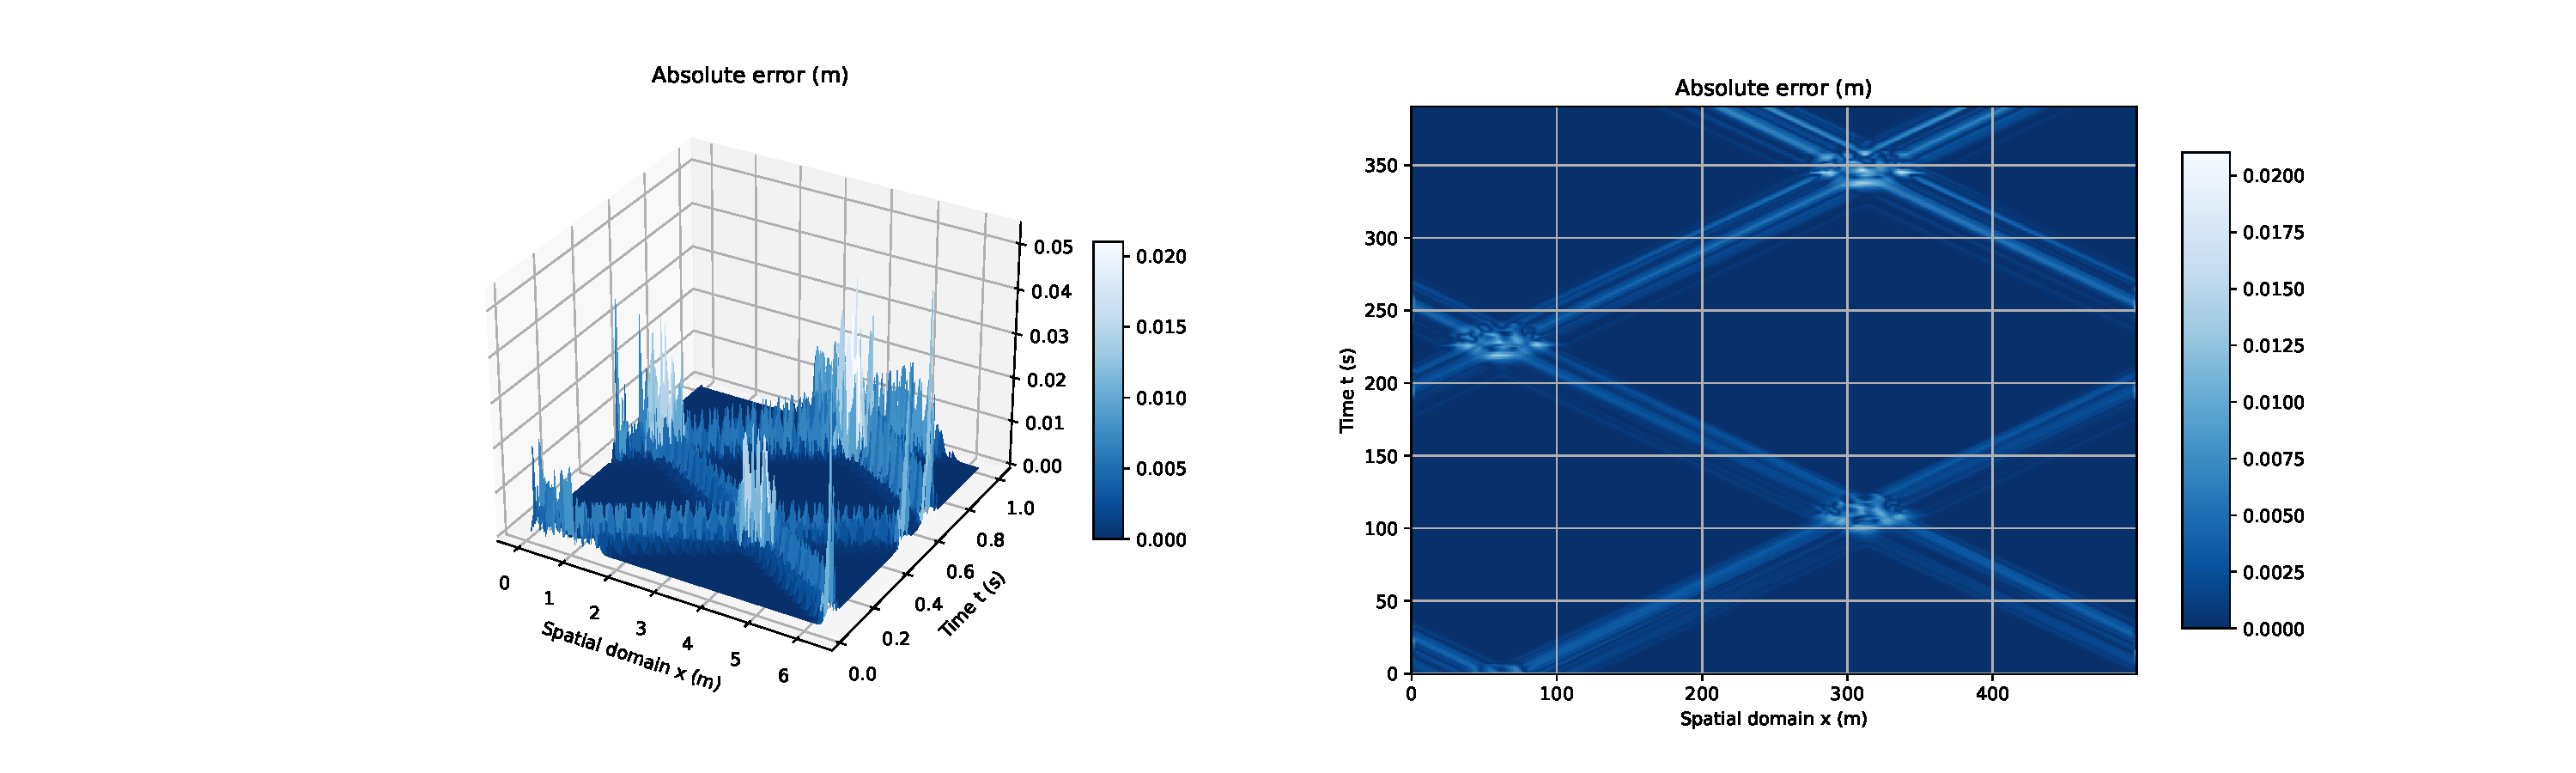
\includegraphics[width=\textwidth]{C:/Users/Matteo/Shallow-Water-Equations/plots/1D_CNN_sphere_error_sigma=2.pdf}
    \caption{Error plots for the predictions of the CNN model for solving the 1D LSWE on a sphere.}\label{fig:1D_CNN_sphere_error}
\end{figure}
In \autoref{fig:1D_CNN_sphere_error}, we see that errors are largest at the sharp edges of the solution.
The predictions for some given time steps are shown in \autoref{fig:1D_CNN_sphere_pred_timesteps_sphere_sigma=2}.
\begin{figure}[H]
    \centering
    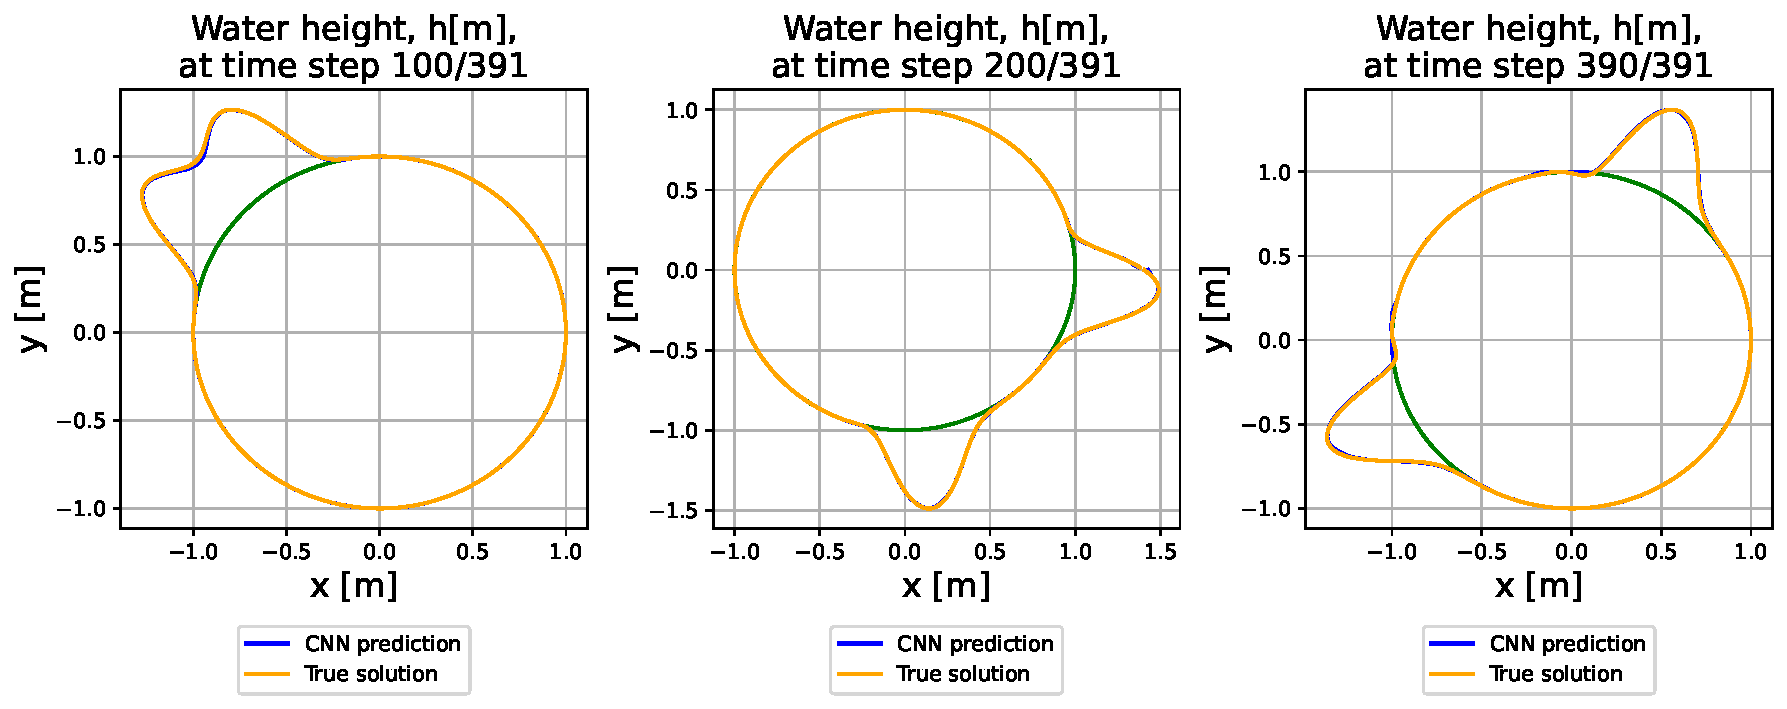
\includegraphics[width=0.9\textwidth]{C:/Users/Matteo/Shallow-Water-Equations/plots/1D_CNN_sphere_pred_timesteps_sphere_sigma=2.pdf}
    \caption{Predictions for the spherical 1D LSWE using the CNN model for some given time steps.}\label{fig:1D_CNN_sphere_pred_timesteps_sphere_sigma=2}
\end{figure}
From \autoref{fig:1D_CNN_sphere_pred_timesteps_sphere_sigma=2}, we see that the predictions capture the waves.
Comparing this to \autoref{fig:1D_CNN_sphere_error}, the error distribution seems reasonable, as the solution remains largely constant except in the areas with the waves, where the errors occur.

\subsubsection*{FNO model}
The FNO model consists of an input channel, 64 hidden channels and an output channel. We use a Fourier basis with 16 modes and a batch size of 32.
The model is trained using the Adam optimizer with a learning rate of $0.001$ and the critera is to minimize the mean squared error (MSE).
The model is trained on the data from $t = 0$ s to $t = 0.6$ s, validated on the data from $t = 0.6$ s to $t = 0.8$ s, and tested on the data from $t = 0.8$ s to $t = 1.0$ s.
The model is trained for $200$ epochs, where the current best model is saved throughout the training.
The training and validation loss is shown in \autoref{fig:1D_FNO_sphere_loss}.
\begin{figure}[H]
    \centering
    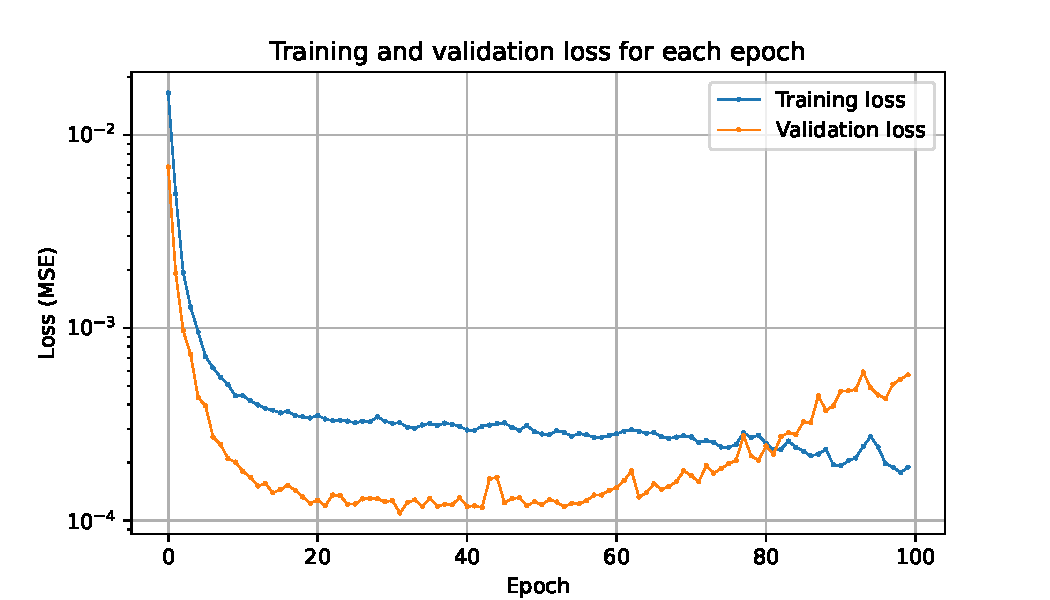
\includegraphics[width=0.7\textwidth]{C:/Users/Matteo/Shallow-Water-Equations/plots/1D_FNO_sphere_loss.pdf}
    \caption{Training and validation loss for the FNO model for the spherical 1D LSWE.}\label{fig:1D_FNO_sphere_loss}
\end{figure}
\autoref{fig:1D_FNO_sphere_loss} shows that the training and validation loss decrease over the epochs, indicating that the model is learning the dynamics of the solution.
We see that after some time the validation loss increases, indicating that the model is overfitting the training data.
This also shows why it can be beneficial to save the current best model throughout the training phase.
The error plots are shown in \autoref{fig:1D_FNO_sphere_error_sigma=2}.
\begin{figure}[H]
    \centering
    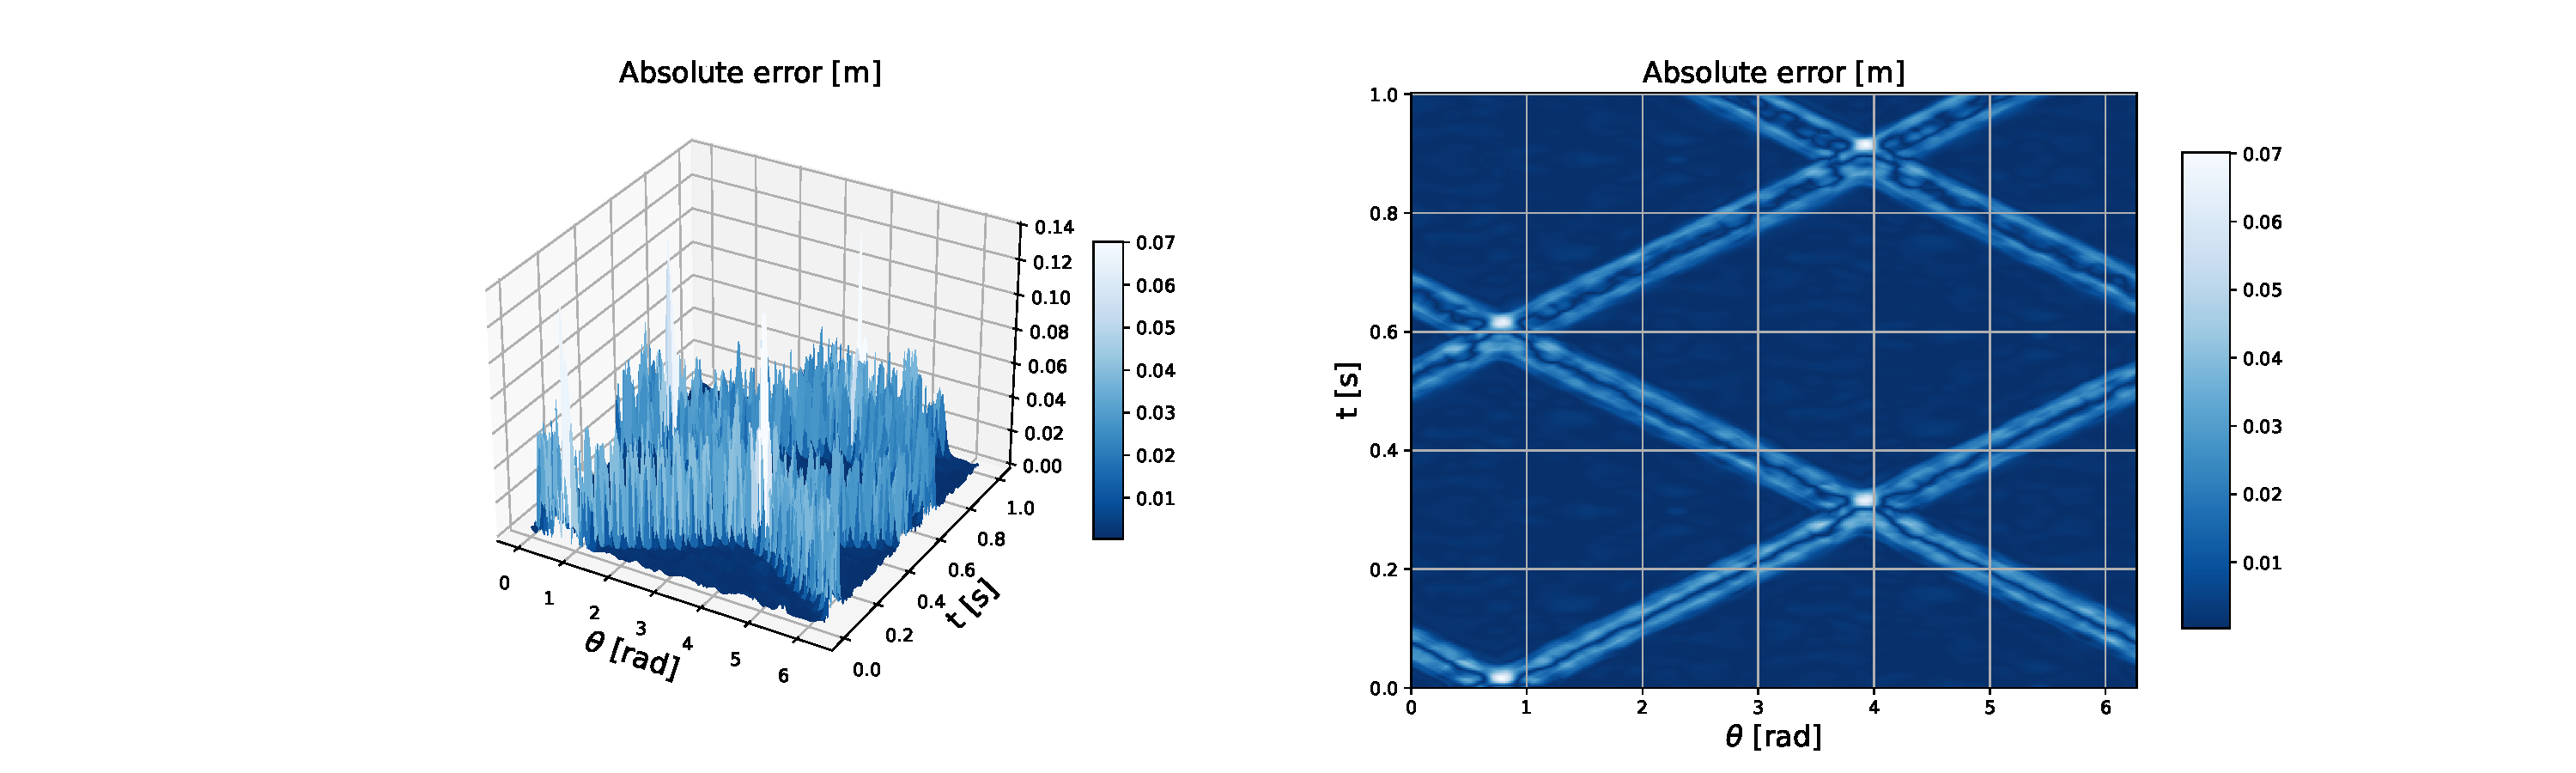
\includegraphics[width=\textwidth]{C:/Users/Matteo/Shallow-Water-Equations/plots/1D_FNO_sphere_error_sigma=2.pdf}
    \caption{Error plots for the predictions of the 1D linearized spherical SWE.}\label{fig:1D_FNO_sphere_error_sigma=2}
\end{figure}
Similar to the CNN model, we observe from \autoref{fig:1D_FNO_sphere_error_sigma=2} that the error is largest at the edges of the solution, where the waves are present.
The predictions for some given time steps are shown in \autoref{fig:1D_FNO_sphere_pred_timesteps_sphere_sigma=2}.
\begin{figure}[H]
    \centering
    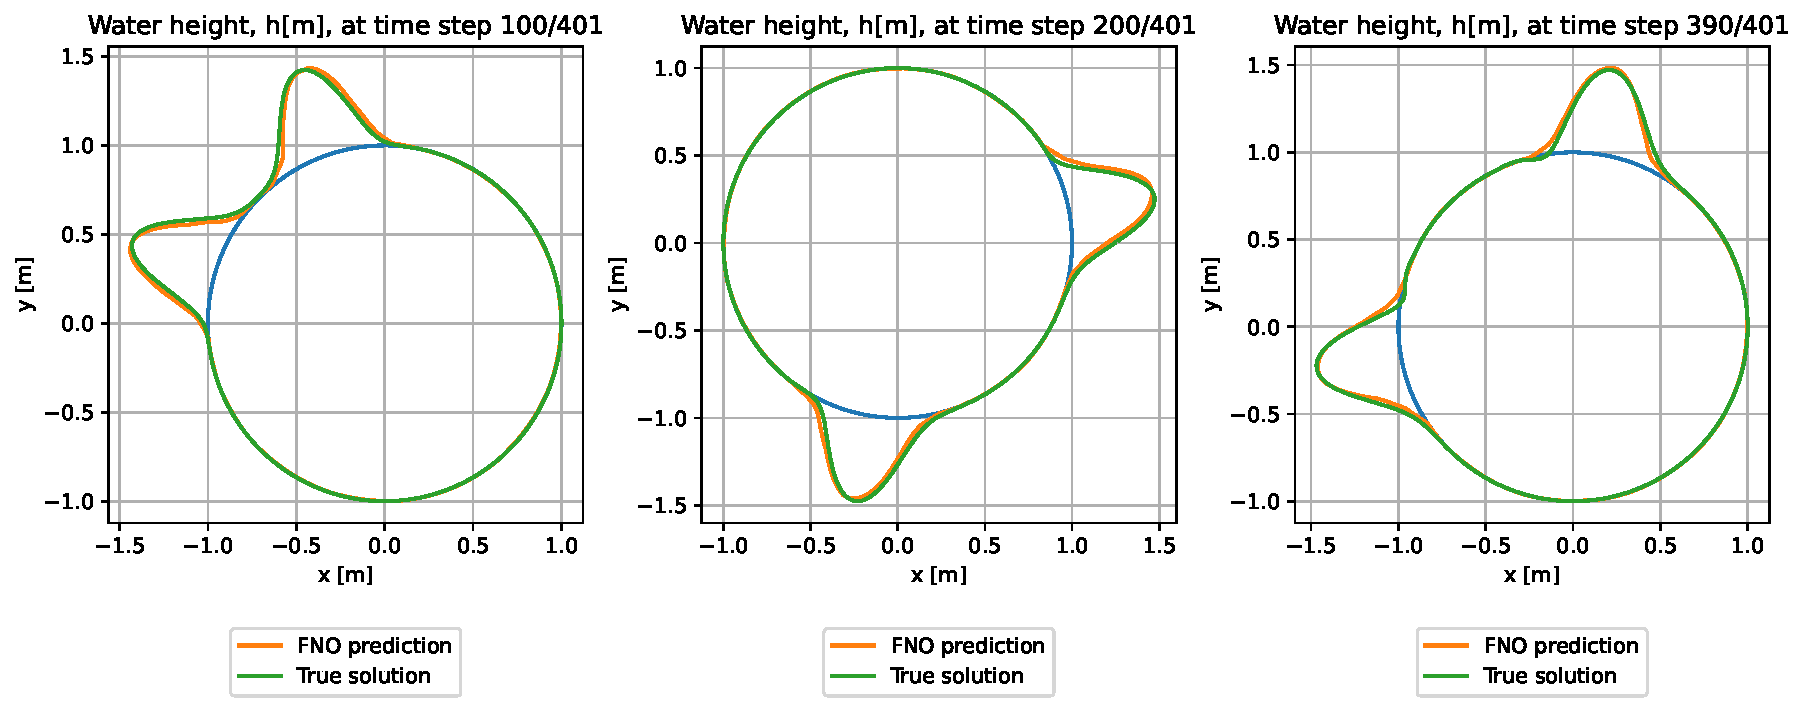
\includegraphics[width=0.9\textwidth]{C:/Users/Matteo/Shallow-Water-Equations/plots/1D_FNO_sphere_pred_timesteps_sphere_sigma=2.pdf}
    \caption{Predictions for the 1D LSWE on a sphere using the FNO model for some given time steps.}\label{fig:1D_FNO_sphere_pred_timesteps_sphere_sigma=2}
\end{figure}
\autoref{fig:1D_FNO_sphere_pred_timesteps_sphere_sigma=2} demonstrates that the FNO model overall captures the waves, but has some minor delays, which was not present in the CNN model.

\subsubsection*{Comparison}
To compare the performance of the CNN and the FNO model, we consider the MSE and MAE for the predictions of the 1D spherical LSWE, as well as the training time for the models.
We are also interested in measuring how the models handle sharp edges in the solution.
Therefore, we introduce two new initial conditions for the water height $h$, as described in~\eqref{eq:1D_swe_spherical_ic}, with $\sigma = \frac{\pi}{8}$ and $\sigma = \frac{\pi}{32}$.
This is done to see how the models perform for different types of initial conditions, depending on how smooth or steep the solution is.
The results are summarized in \autoref{tab:results_spherical_1D_comparison}.
\begin{table}[H]
    \centering
    \small % Reduce font size
    \begin{tabular}{c|ccc|ccc|ccc}
        \hline
        Model & \multicolumn{3}{c|}{$\sigma = \pi/8$} & \multicolumn{3}{c|}{$\sigma = \pi/16$} & \multicolumn{3}{c}{$\sigma = \pi/32$} \\
        \cline{2-10}
        & MSE & MAE & Time [s] & MSE & MAE & Time [s] & MSE & MAE & Time [s] \\
        \hline
        CNN & 
        \input{C:/Users/Matteo/Shallow-Water-Equations/saved_results/1D_CNN_sphere_sigma=1_MSE_test.txt} &
        \input{C:/Users/Matteo/Shallow-Water-Equations/saved_results/1D_CNN_sphere_sigma=1_MAE_test.txt} &
        \input{C:/Users/Matteo/Shallow-Water-Equations/saved_results/1D_CNN_sphere_sigma=1_time.txt} &
        \input{C:/Users/Matteo/Shallow-Water-Equations/saved_results/1D_CNN_sphere_sigma=2_MSE_test.txt} &
        \input{C:/Users/Matteo/Shallow-Water-Equations/saved_results/1D_CNN_sphere_sigma=2_MAE_test.txt} &
        \input{C:/Users/Matteo/Shallow-Water-Equations/saved_results/1D_CNN_sphere_sigma=2_time.txt} &
        \input{C:/Users/Matteo/Shallow-Water-Equations/saved_results/1D_CNN_sphere_sigma=3_MSE_test.txt} &
        \input{C:/Users/Matteo/Shallow-Water-Equations/saved_results/1D_CNN_sphere_sigma=3_MAE_test.txt} &
        \input{C:/Users/Matteo/Shallow-Water-Equations/saved_results/1D_CNN_sphere_sigma=3_time.txt} 
        \\ 
        \hline
        FNO & 
        \input{C:/Users/Matteo/Shallow-Water-Equations/saved_results/1D_FNO_sphere_sigma=1_MSE_test.txt} &
        \input{C:/Users/Matteo/Shallow-Water-Equations/saved_results/1D_FNO_sphere_sigma=1_MAE_test.txt} &
        \input{C:/Users/Matteo/Shallow-Water-Equations/saved_results/1D_FNO_sphere_sigma=1_time.txt} &
        \input{C:/Users/Matteo/Shallow-Water-Equations/saved_results/1D_FNO_sphere_sigma=2_MSE_test.txt} &
        \input{C:/Users/Matteo/Shallow-Water-Equations/saved_results/1D_FNO_sphere_sigma=2_MAE_test.txt} &
        \input{C:/Users/Matteo/Shallow-Water-Equations/saved_results/1D_FNO_sphere_sigma=2_time.txt} &
        \input{C:/Users/Matteo/Shallow-Water-Equations/saved_results/1D_FNO_sphere_sigma=3_MSE_test.txt} &
        \input{C:/Users/Matteo/Shallow-Water-Equations/saved_results/1D_FNO_sphere_sigma=3_MAE_test.txt} &
        \input{C:/Users/Matteo/Shallow-Water-Equations/saved_results/1D_FNO_sphere_sigma=3_time.txt} 
        \\ 
        \hline
    \end{tabular}
    \caption{Test loss in terms of MSE and MAE, and time for training the models for the 1D spherical SWE.}\label{tab:results_spherical_1D_comparison}
\end{table}
From \autoref{tab:results_spherical_1D_comparison} we observe that the CNN model is slightly faster and achieves a lower MSE and MAE than the FNO model across all three initial conditions.
However, the difference for $\sigma = \pi/32$ is minimal, suggesting that the FNO model performs better at capturing steeper edges in the solution.
Additionally, the FNO model exhibits more stable performance with new initial conditions, while the CNN model shows more variation.

It is also notable that the MAE is generally higher than the MSE and increases as $\sigma$ decreases.
This difference highlights that the MAE places greater emphasis on small errors compared to the MSE.

